\chapter{Computer architecture review}
\label{ch:comparch}

% \begin{goals}
%   \begin{enumerate}
%   \item \textbf{Describe} the basic arrangement of modern computing devices.
%   \item \textbf{Explain} the key features of modern CPUs.
%   \end{enumerate}
% \end{goals}

% \begin{reading}
%   Review previous computer architecture notes.
% \end{reading}

\section{CPU components}

\begin{figure}[htbp]
  \centering
  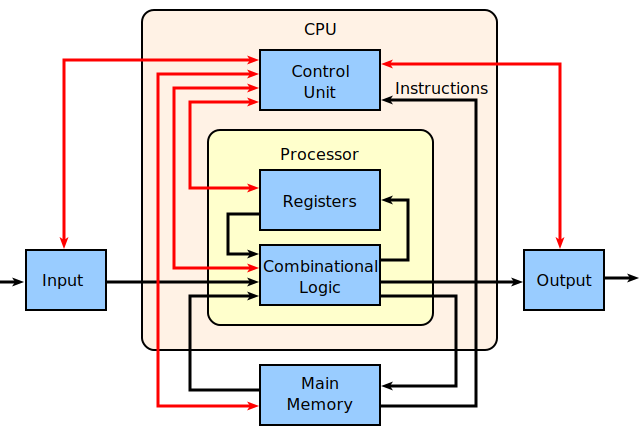
\includegraphics[width=0.5\linewidth]{cpu}
  \caption{CPU (Wikipedia)}
  \label{fig:cpu}
\end{figure}

Key components:

\begin{description}
\item[Control unit] decodes \textit{instructions} to control the operation of the CPU.
\item[Arithmetic Logic Unit] performs arithmetic (addition, subtraction) and logical (AND, OR, NOT, XOR) operations.
\item[Registers] are used as a working variable store for the CPU, particularly ALU operations.
  \begin{description}
  \item[Program counter (PC)] stores the address of the next instruction to be executed.
  \item[Stack pointer (SP)] stores the memory address of the \textit{call stack} (later!)
  \item[Flags] indicate certain conditions that are often errors, e.g. division by zero. 
  \end{description}
\end{description}

\section{Fetch-execute cycle}

\section{Instruction set architecture}

\begin{description}
\item[CISC] --- complex instructions, designed for humans, usually memory-register, variable number of cycles per instruction
\item[RISC] --- simple instructions, designed for compilers, load-store, every instruction executes in a single cycle.
\end{description}

\section{Stored program architectures}

\begin{description}
\item[von Neumann] instructions and data occupy same address space.
\item[Harvard] instructions and data are in separate memory address spaces. 
\end{description}

\section{Interrupts}
\label{sec:interrupts}


